%\graphicspath{./Chapters/appendix1/figs/}


In this section I will describe the background and the current status of the fusion energy research related to this PhD thesis.
\section{Fusion energy} \label{Fusion_energy}

In a fusion reaction two light nuclei fuse and a heavier nucleus is generated. The energy released in the reaction depends on how strongly protons and neutrons are bound in the nucleus of reactant and products. This strength is expressed by the average binding energy per nucleon, that is the energy necessary to decompose one nucleus over the number of nucleons. The energy released by the nuclear reaction is given by the difference of the total binding energy in the products minus the reactant. \autoref{fig:binding_energy} shows that it is possible to obtain energy in two ways: fusion and fission. In fusion, the lighter the reactant the larger the energy released.

\begin{figure}
	\centering
	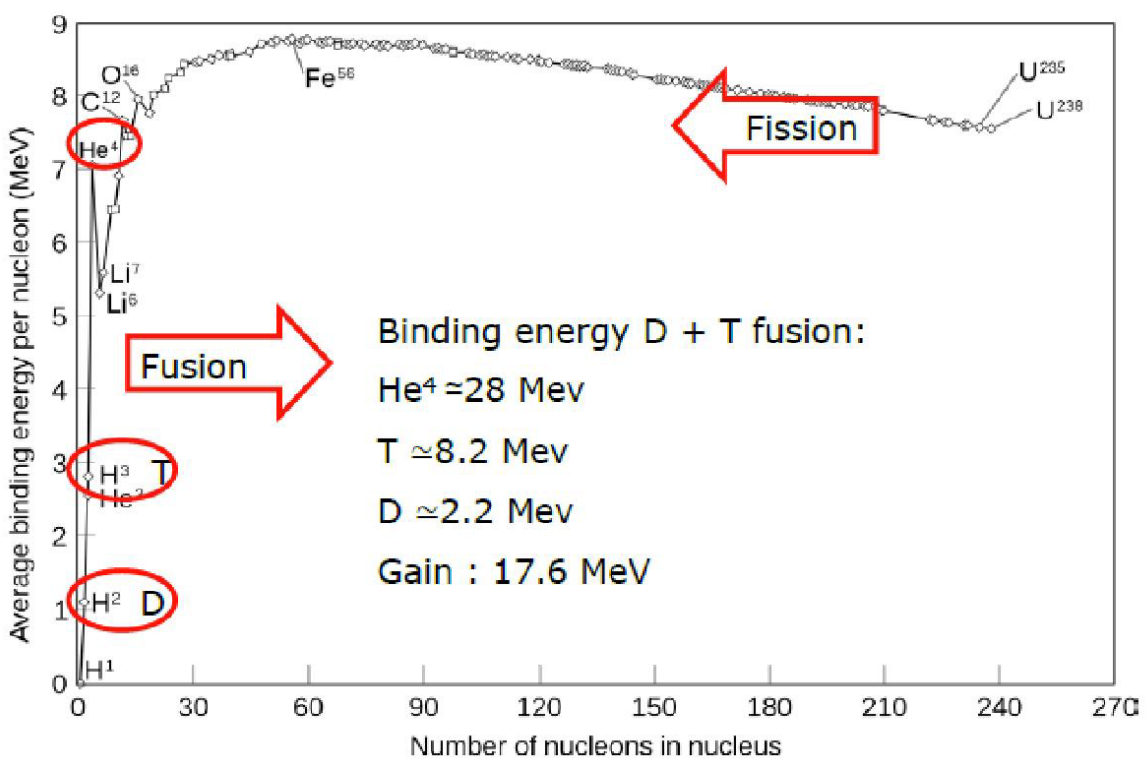
\includegraphics[width=\linewidth]{Chapters/chapter1/figs/binding energy.PNG}
	\caption{Average binding energy per nucleon \cite{YanNingNaulinVolkerWanBaonianXu2014}}
	\label{fig:binding_energy}
\end{figure}

Another factor to consider in comparing different fusion reactions is the likelihood of the reaction to happen. This is characterised by the fusion cross section, that depends on the kinetic energy of the incident particle. Considering an ensemble of particles this kinetic energy translate in temperature. The lower the temperature for which the cross section reaches its peak the easier to achieve fusion.
For this and other reasons the reaction that is the main focus of current research is the fusion of deuterium and tritium to helium: \cite{Miley1974}

\begin{equation}
{ }^2_1 D+ { }^3_1T \leftarrow { }^4_2He+{ }^1_0n
\label{eq:fuse}
\end{equation}

In this reaction are released 3.5MeV in kinetic energy of the alpha particle and 14.1MeV in the neutron. Tritium is not available in nature because it is radioactive with a short half life, so it must be produced. It is foreseen to produce it using the neutron released in reaction \ref{eq:fuse} in the reactions \ref{eq:fuse1} and \ref{eq:fuse2}

\begin{equation}
{}^{6}Li + n \leftarrow {}^{4}He +T +4.78MeV
\label{eq:fuse1}
\end{equation}

\begin{equation}
{}^{7}Li + n \leftarrow {}^{4}He +T +n +2.47MeV
\label{eq:fuse2}
\end{equation}

The initial fuels in this cycle then are deuterium and lithium, both widely available in nature.

\section{Plasma confinement}
%\hl{triple product, H mode, SOL, ELMs}

The temperatures that are relevant for fusion application are measured in keV, that correspond to millions of °C. At these temperatures matter is in the state of plasma, meaning that atoms are ionised and nuclei and electrons can move freely. These temperatures are of the same order of magnitude of the centre of the Sun. No material can withstand them so special techniques must be adopted to confine the reactant long enough for a significant fraction to fuse. The most important figure of merit of the achieved confinement is the fusion triple product, related to Lawson criteria, that returns the minimum product of plasma density, temperature and confinement time to achieve ignition (\autoref{eq:fuse3}). Ignition is the condition when the fusion power output is sufficient to maintain a constant temperature against all losses without external heating.

\begin{equation}
{n_e} {\tau }_{E} T_e  >=  5\cdot{10}^{21}{ m }^{ -3 }skeV
\label{eq:fuse3}
\end{equation}

The most viable way to maintain this environment is expected to be
through magnetic confinement, and specifically the tokamak (Magnetic Confinement Fusion, MCF).
In MCF the fuel is confined in plasma state thanks to its behaviour when exposed to electromagnetic fields. Every electrically charged particle is subject to Lorentz force:


\begin{equation}
F = q ( E+ vxB )
\label{eq:lorentz}
\end{equation}

In the presence of a magnetic field the particle gyrate with a circular motion in the direction perpendicular to field lines and is unperturbed in the parallel direction. In a tokamak the plasma is arranged in a doughnut shape, closely surrounded by two main set of coils: the toroidal field coils that generate the toroidal magnetic field and the central solenoid that with a time varying current induces a current through the plasma that generates the poloidal magnetic field. The toroidal geometry cause drifts in the plasma that would cause it to quickly reach the walls and cool down. To stabilise the plasma and shape it as requested other coils have to be added.\cite{Chen1974} The magnetic field generated in this way is composed of concentric flux surfaces that expand to the coils. The final configuration is outlined in \autoref{fig:mcf}. Shown in pink is a magnetic surface, that is the set of all the positions a particle can assume when streaming unimpeded following magnetic field line. JET is currently the largest tokamak and has achieved triple products higher than $10^{21} m^{-3}skeV$ in 1997 \cite{Gormezano1998} and recently the record for fusion energy produced of 59MJ. \cite{Gibney2022}

\begin{figure}
	\centering
	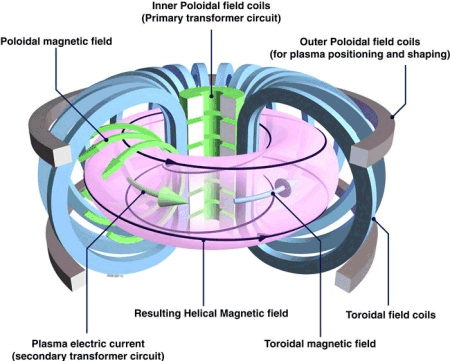
\includegraphics[width=\linewidth]{Chapters/chapter1/figs/mcf.png}
	\caption{Schematic of the main components of a tokamak \cite{CulhamCentreforFusionEnergy2018}}
	\label{fig:mcf}
\end{figure}

The plasma can move freely along the field lines and slowly across it, so in time it drifts from the centre toward the wall via cross field transport caused by collisions and turbulence. One of the important evolutions of the tokamak design is to add a coil parallel to the plasma with a current in the opposite direction. This changes the magnetic configuration in such a way that the core of the plasma is not any more in direct contact with a solid limiter. The first magnetic surface that crosses solid surfaces from the core is referred as Last Closed Flux Surface (LCFS) or separatrix and where the poloidal field goes to zero is the x-point. The separatrix crosses the solid surfaces in well defined regions, called divertor targets. The plasma that escapes from the core (which state is usually referred to as "upstream") reaches the separatrix and then follows the magnetic field around the core and reaches the targets. In this way the core is shielded from the impurities generated by the plasma/surface interaction and can efficiently expel the fusion products. This motion along field lines is much faster than across and it is associated with a layer out of the LCFS called Scrape-Off Layer (SOL). The time a particle needs to cross the plasma from the centre and reach the wall defines the confinement time.

\section{H-mode}
A way to limit cross field transport in the core region and move towards ignition is to operate in the so called H mode. This regime is reached when the energy flux across the separatrix is increased over a threshold that depends on the discharge conditions.\cite{Ryter1998} The physics behind the specific value of the L-H threshold is still not fully understood, but its effect is to induce a transport barrier at the edge of the core plasma. This barrier strongly reduces the anomalous transport due to turbulence in a thin region around the core, allowing for a better energy and particle confinement there. One drawback of the H-mode is that it causes cycles of accumulation of energy in the core and sudden release as bursts of hot plasma. These so called Edge Localised Modes (ELMs) cause transient high particle and thermal flux on the target. Moreover in order to sustain the H-mode a certain amount of power must cross the separatrix, otherwise the H-L back transition can occur. This constitutes a lower bound to the heat and particles that need to be dissipated from the separatrix to the target.

\section{The exhaust problem}
%\hl{thin SOL, melting/erosion}

The issue that arises with the divertor configuration is that the SOL is  very narrow, of the order of mm, and all the exhaust heat is delivered to a small area of the target. For ITER, a fusion device in construction in France that will be a step closer to a power production device, this heat is in the order of $GW/m^2$. The maximum power that can be removed from a surface with current technologies is $10-20MW/m^2$.\cite{Lipschultz2018} If the heat to the target is not mitigated this will pose a serious limitation on its lifetime and the amount of impurities reaching the plasma, making impossible profitable operations. 
Sputtering is the phenomenon of emission of one or multiple atoms from a solid surface caused by interaction with an ion. This happens even for heat fluxes much lower than what is required for melting the surface. There are various types of possible interactions but, as a whole, larger the energy of the ion larger number of atoms are sputtered from the surface. The local interaction of the plasma with a solid surface creates a sheath where the ions are accelerated towards the surface up to the sound speed $c_s \approx \sqrt{\frac{2kT}{m_i}}$ (where $m_i$ is the ion mass and $k$ the Boltzmann constant), exacerbating sputtering. The sputtered atoms can end in the plasma, polluting it, or be redeposited to the target, changing its composition and properties. The sputtering can be so severe to be the main limiting factor of the lifetime of the plasma facing components.

\section{Divertor shaping}
%\hl{total/poloidal flux expansion}

The heat and particle flux can be reduced by tilting the target with respect to the separatrix and by locally reducing the magnetic field, thus spreading the heat on a larger surface.
Under investigation are different divertor designs (see some on \autoref{fig:divertor_geometry}) with the purpose, among others, to ease the thermal burden on the target

\begin{figure}
	\centering
	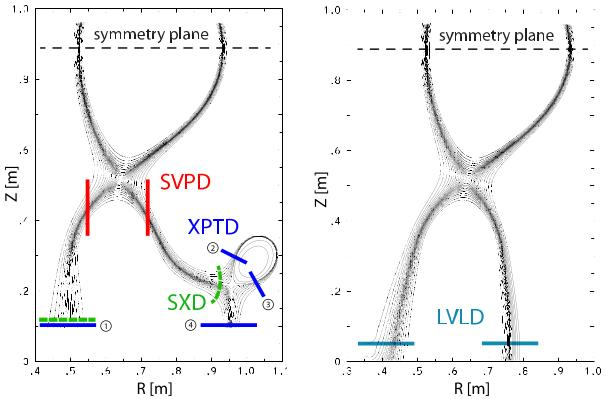
\includegraphics[width=\linewidth]{Chapters/chapter1/figs/divertor geometry.jpg}
	\caption{Example of different divertor configurations. Left:Standard Vertical Plate Divertor (SVPD), Super-X Divertor (SXD) and X-point Divertor (XPTD). Right: Long Vertical Leg Divertor (LVLD) \cite{Umansky2017}}
	\label{fig:divertor_geometry}
\end{figure}

The two above mentioned effects combined lead to a reduction of the heat flux density around 20 times for a tokamak of SVPD divertor type like will be on ITER, still short of another 10 times reduction needed to respect the 10-20 MWm-2 limit. The divertor configuration introduces an asymmetry in the toroidal geometry due to the two targets located at different radii. In terms of energy and particle redistribution in the SOL the inner target will receive a higher ion flux and lower energy flux compared to the outer one. As it will become clear later, on the inner target this causes stronger recycling and eases the thermal load, while the outer target is normally subjected to more severe conditions. [\cite{Potzel2014} and references there therein]

\section{Radiative dissipation scenario}
%\hl{energy removal --> radiative scenario, impurities}

Another way to decrease the heat flux to the target is to induce radiation in the SOL.
Radiation occurs naturally in plasmas and it depends greatly on temperature and density of each specie. When an atom is not yet fully ionised the electronic levels can be excited by collision and de-excite emitting a photon. The ionised atoms can recombine with free electrons and release a photon too. The energies at which these effects are more likely correspond to the peaks in the curves in \autoref{fig:loss_curve}. If the temperature is so high that atoms are fully ionised the only radiative mechanism is Bremsstrahlung radiation, that is much less efficient. This corresponds to the monotonic increasing right part of the curves in \autoref{fig:loss_curve}.

\begin{figure}
	\centering
	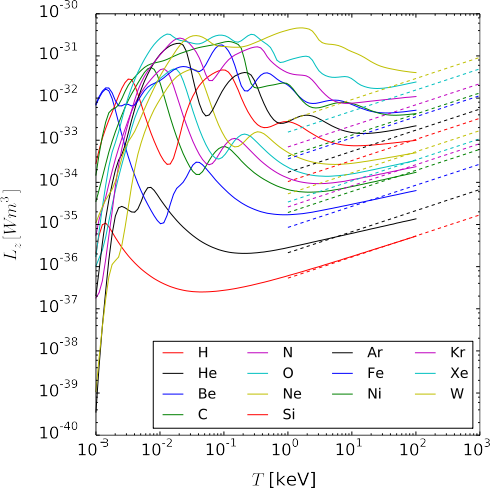
\includegraphics[width=\linewidth]{Chapters/chapter1/figs/loss curve.png}
	\caption{Loss function data from the ADAS data base (solid lines) for the different elements \cite{Lux2015}}
	\label{fig:loss_curve}
\end{figure}

At the temperatures of interest in the SOL (100s of eV\cite{Pacher2011}) hydrogen is fully ionised and radiates weakly. With the addition of impurities sputtered from the wall or specifically seeded in the discharge the energy can be transferred from the plasma to the impurities and then radiated. This mechanism can be exploited to dissipate a significant amount of power from the core and edge of the plasma, but also the SOL. This regime is referred to as the radiative scenario.


\section{Detachment}\label{Detachment}
%\hl{particle removal -> recycling, detachment}

At low upstream densities the plasma that enters the SOL can flow relatively unimpeded towards the target. The temperature in the SOL is about constant and the particle flux is limited only by the sheath condition (e.g. "sheath-limited"). By increasing the core and SOL density plasma heat flux conductivity decreases (e.g. "conduction limited"), leading to negative gradients of the temperature and positive of the density, with an almost uniform pressure. In this regime the heat flux to the target is the sum of the component parallel to field lines $q_{par}$, the orthogonal one $q_{ort}$ and a component given by the energy released with recombination $q_{rec}$, given by  \autoref{eq:detachment}.

\begin{equation}
\begin{aligned}
{ q } _{ par } =& { n } _{ e,t } { c } _{ s } {  \gamma  } _{ sh }{ k } _{ B }{ T } _{ e,t } \; \alpha \; { p } _{ e,t }{{ T } _{ e,t }}^{0.5 } \\
{ q } _{ ort } =& { q } _{ par } \left( \frac {{ B } _{ p }} {{  B  }_{ \phi  }}   \right) _{ t} \; \alpha \; { p } _{ e,t }{{ T } _{ e,t }}^{0.5 } \\
{ q } _{ rec } =& { n } _{ e,t } { c } _{ s } {  E  } _{ pot } \; \alpha \; { p } _{ e,t }{{ T } _{ e,t }}^{-0.5 }
\end{aligned}
\label{eq:detachment}
\end{equation}

where $\gamma_{sh}$ is the heat sheath transmission factor, $n_{e,t}$ and $T_{e,t}$ are the electron density and temperature in front of the target, $c_s$ is the sound speed, $B_p$ and $B_{\Phi}$ are the poloidal and toroidal magnetic field and $E_{pot} \approx 15.8 eV$ is the potential energy released per ion when recombining to neutral deuterium molecules on the target plate. \cite{Reimold2015} The temperature cannot be indefinitely reduced because of operational limits like the Greenwld limit.\cite{Greenwald1988} Moreover, a reduction of the temperature does not alone guarantees a decrease of the heat flux.  One possible solution to achieve it is to cause gradients of temperature and pressure along the field lines in the SOL. This should be done in such a way to minimize the impact on the core plasma.

A way to achieve this is to induce plasma detachment. This phenomenon has been observed in a series of tokamaks [\cite{Reimold2015} and references therein] and can be induced by impurity seeding or fuelling.
In an attached regime the plasma streams through the SOL and reaches the target. At the target the charged particles recombine and become neutrals. They are generated in an excited state therefore a strong radiation at the strike points. The neutrals are not bound by magnetic fields, and can move freely until they collide with other neutrals or particles from the plasma. A neutral can then re-ionise and stream along field lines, returning to the target or entering the plasma again. This process is called recycling and the region of the leg where it occurs the ionisation or recycling region.

If the density in the SOL is high enough the neutrals generated by the plasma streaming outward will interact mainly in the SOL and the plasma will loose part of its energy and momentum on its way to the target. To further increase the energy loss low Z impurities like Nitrogen can be seeded in the SOL: they will ionise only partially, radiating efficiently at higher temperature than hydrogen or helium. The lower the temperature the higher the energetic ionisation cost. This because lower temperature means smaller progressive excitation by collisions of the bound electron up to ionisation with radiative losses in the process, instead of a single higher energetic collision directly to ionisation. This cause even more radiative cooling. In most cases, and especially if the divertor is baffled like in MAST-U, allowing for a higher neutral density inside, the volumetric ionisation source from neutrals constitute the main source of ions for the target flux.\cite{Krasheninnikov2016,Krasheninnikov2017a,Lipschultz1999} This is referred to as high recycling, where the recycling region constitutes a self-contained system that is supplied from upstream mainly of energy. This is believed to be one of the most important difference between tokamak divertors and linear machines, where the main source of ions is usually the plasma source upstream. Simulations for the linear machine Pilot-PSI,characterised by a very high density, show that ionisation could account for up to a third of the plasma source, but this in  region very close to the source itself.\cite{Jesko2018,Hayashi2016} This, though, was not found when simulating the similarly high density Magnum-PSI, nor experimentally validated yet to the author's knowledge.\cite{Chandra2022}

From detachment experiments it is observed that the particle flux to the target increases with increasing core density. Increasing further the density or impurity seeding the particle flux reaches a maximum and then decreases. This is called rollover and corresponds with the onset of detachment. Other metrics for the detachment offset have been used, as the decrease of the target temperature below a certain threshold\cite{Stangeby2000,Goldston2017}, but the Langmuir probe constitute a direct and simple measurement, hence their widespread use. Pushing the process forward the particle flux decrease and saturates. In the case the plasma could loose all its kinetic energy, or temperature, it still maintains the energy associated with its creation, the ionisation and dissociation energy, $15.8eV$. In a DEMO scale device this residual energy flux would be still high enough to exceed the $10-20 MWm^{-2}$ limit on the target. \cite{Krasheninnikov2017a} To reduce it even further the temperature must drop below $1eV$ to trigger volumetric recombination. This is accompanied by a strong radiation increase from where volumetric recombination occurs. The particle flux drop can continue up to the point that the measured plasma temperature at the target reaches a minimum and the radiating region (radiation front) recedes upstream along the field lines.\cite{Krasheninnikov1999} at different stages in this process different fronts will in turn detach from the target line the ionisation and thermal front.\cite{Hutchinson1994,Loarte1998,Lipschultz2016} The fronts movement comes from the balance between the power and particles entering the SOL with dissipation by radiation and interaction with recycling neutrals.


\section{Atomic and molecular processes}
\hl{
            1. attached $->$ hot $->$ atomic physics
            2. detached $->$ cold $->$ atomic and molecular physics}
\section{The x-point radiator}\label{The x-point radiator}
%\hl{extreme end of detachment before MARFE, increased radiated power}

When a discharge in both L-mode and H-mode is close to the detachment threshold in a tokamak with a conventional divertor configuration and the impurity or core density is increased 4 stages of detachment are defined as per the description in \cite{Reimold2015,Potzel2014}. Here with detachment is intended the particle flux roll over and deviation from the attached case scaling as will be shown later.

\begin{enumerate}
    \item Onset of detachment: the inner target detaches inter-EMLs (even due to recycling and without impurity seeding), the outer target is attached
    \item Fluctuating state: radiative fluctuations in the kHz appear at the X-point, inner target detaches inter-EMLs
    \item Partial detachment at outer target: inner target always detached, outer target detached inter-ELMs, strong radiation at the X-point, fluctuations frequency decrease to ELMs scale, ELMs amplitude decrease.
    \item Complete detachment: inner and outer target always detached, sporadic ELMs, radiator moves from X-point further into the confined plasma
\end{enumerate}

For this type of discharge the radiator close to the X-point appears when detachment starts at the inner target, while it is only enhanced by the detachment on the outer target. Because the parameter of interest is the reduction of thermal flux on the outer target a feature that will always be present in reactor relevant conditions is a strong radiator located close to the X-point.

\section{Effect of X-point radiator}\label{Effect of X-point radiator}
%\hl{poloidal asymmetry, pedestal flattening, loss confinement}


The X-point radiator (XPR) is a region of steep temperature gradient, where the temperature goes from that of the hot upstream plasma from the core to the cold region where ion / neutral interactions dominate. The presence of such a thing at or inside the separatrix can lead to confinement degradation. In this context what is referred as confinement H98 is the ratio of the actual energy confinement time $\tau_{th}$ over a reference. The reference is a confinement time from a scaling law obtained fitting the confinement time of many tokamak experiments in a certain operating mode. For ELMy H-mode the scaling law mostly used is the ITER Physics Basis (IPB) 98(y,2).\cite{Doyle2007} For L-mode the ITERL-97P scaling can be used. \cite{Kaye1997} The scalings are given by \autoref{eq:h98y2} and \ref{eq:l97}. For spherical tokamaks an H-mode \cite{Kaye2006} and MAST L-mode \cite{Kaye2021} scaling are given in \autoref{eq:HST}, \ref{eq:LST} respectively.


\begin{equation}
{ H }_{ 98 }={\tau }_{ th }/{\tau }_{ th,98y2 } \; , \; {\tau }_{ th,98y2 }=0.0562 {{ I }_{ P }}^{ 0.93} {{ B }_{ t }}^{ 0.15} {{ n }_{ 19 }}^{ 0.41} {{ P }_{ L }}^{ -0.69} {{ R }_{  }}^{ 1.97} {{ \varepsilon  }_{  }}^{ 0.58} {{ \kappa  }_{ a }}^{ 0.78} {{ M }_{  }}^{ 0.19}
\label{eq:h98y2}
\end{equation}

\begin{equation}
{ L }_{ 97 }={\tau }_{ th }/{\tau }_{ th,97P } \; , \; {\tau }_{ th,97P }=0.037 {{ I }_{ P }}^{ 0.74} {{ B }_{ t }}^{ 0.2} {{ n }_{ 19 }}^{ 0.24} {{ P }_{ L }}^{ -0.75} {{ R }_{  }}^{ 1.69} {{ \varepsilon  }_{  }}^{ 0.31} {{ \kappa  }_{ a }}^{ 0.67} {{ M }_{  }}^{ 0.26}
\label{eq:l97}
\end{equation}


\begin{equation}
{ H }_{ ST }={\tau }_{ th }/{\tau }_{ th,HST } \; , \; {\tau }_{ th,HST }=0.066 {{ I }_{ P }}^{ 0.53} {{ B }_{ t }}^{ 1.05} {{ n }_{ 19 }}^{ 0.65} {{ P }_{ heat }}^{ -0.58} {{ R }_{  }}^{ 2.66} {{ \kappa  }_{ a }}^{ 0.78}
\label{eq:HST}
\end{equation}

\begin{equation}
{ L }_{ ST }={\tau }_{ th }/{\tau }_{ th,LST } \; , \; {\tau }_{ th,LST }=0.153 {{ I }_{ P }}^{ 1.01} {{ B }_{ t }}^{ 0.7} {{ n }_{ 19 }}^{ -0.07} {{ P }_{ L }}^{ -0.37}
\label{eq:LST}
\end{equation}

With $I_P$ plasma current in $MA$, $B_t$ toroidal magnetic field in $T$, $n^{19}$ averaged electron density in units of $10^{19} \#/m^3$, $P_L=P-dW/dt$ power loss in $MW$ with $P$ heating power and $W$ stored energy, $R$ major radius, $a$ minor radious, $\varepsilon=a/R$ inverse aspect ratio, $\kappa _a$ elongation, $M$ ion mass number in $amu$.
It is possible to calculate the energy confinement time from magnetic coils measurements and the energy transferred to the plasma as heating ($P_{heat}$). $\tau_{th}$ is defined by 

\begin{equation}
\begin{split}
\frac {dW} {dt}={P}_{heat} - \frac {W} {\tau }_{ th } \; , \; W=\frac { 3} {2} \langle p \rangle V \; , \; \langle p \rangle = \frac {{ \mu }_{ 0 } {{ I }_{ p }}^{ 2 } { \beta }_{ p }} { 8 {\pi}^{2} {a}^{2}  } \\ {\beta }_{ p } = \langle \frac { n {k}_{B} T} { {{B}_{p}}^{2} /(2 {\mu}_{0}) } \rangle \; , \; {P }_{ heat }={ P }_{ ohmic }+{ P }_{ NBI }+{ P }_{ RF }
\label{eq:tau}
\end{split}
\end{equation}


With $V$ plasma volume, $\langle p \rangle$ volume-averaged plasma kinetic pressure, ${{ \beta }_{ p }}$ poloidal beta, $B_p$ poloidal magnetic field, $a$ minor radius, $P_{ohmic}$, $P_{NBI}$, $P_{RF}$, power transferred to the plasma by ohmic heating, neutral beam injector and radio frequency respectively. \cite{SalarElahi2010,Fallis2013} The confinement loss is usually done comparing before and after the appearance of the X-point radiator, or with a series of discharges in similar conditions but without and without X-point radiator.
The confinement degradation can be due to the direct cooling caused by the cold region (e.g. poloidal temperature gradients to drive power to that location \cite{Lipschultz1998} ) or to easier penetration of impurities in the core [\cite{Lipschultz2016} and references therein]. The degradation significantly affects the outer part of the core region with significant reduction of temperature, pressure and an increase of density. \cite{Kallenbach2015a}  It was found on some experiments that the inner core (ratio of poloidal magnetic flux over poloidal magnetic flux at the separatrix $ \rho _{pol}<0,8-0,5 $) is only marginally effected. [\cite{Reinke2013} and reference therein]It is therefore suggested that the gradients lost on the pedestal region could be recovered in a portion of plasma $0,8< \rho _{pol}<0,95$. \cite{Reimold2015}

The X-point radiator will also have the effect of radiating a substantial fraction ($75-90\%$ of the heating power achieved \cite{Bernert2017}) of the total $ \alpha $ particles / heating power out of the separatrix and could cause the H-L transition. This is anyway not a major risk for ITER and larger machines, because the power crossing the separatrix is expected to be significantly larger that the threshold requirement. It has been in fact considered to seed a higher-Z impurity in the plasma to enhance core radiation (radiative mantle) and lower the power needed to be exhausted through the separatrix to about the minimum for the L-H transition. Then a lower-Z impurity will be fed to radiate in the divertor. [\cite{Kallenbach2015a,Reinke2013} and reference therein]


There are two active areas of research to limit confinement losses with XPR.

One is in trying to achieve detachment but not allow the radiator moving all the way to the X-point and cause confinement degradation. The main difficulty in achieving this is that, for standard divertor geometries the operational window of any given control parameter to move the radiator from target to X-point is very narrow. Considerable effort has been put forward to find a predictive model. The thermal front model proposed by Lipschultz \cite{Lipschultz2016} is a 1D model that, balancing input / output power on the thermal front (edge of the radiator toward the core), tries to identify the operational window of a control parameter and its stability for given plasma / magnetic configuration. This model finds that for all the control variables analysed the operational window widens for increasing ratio of X-point over target magnetic field $B_x/B_t$ and ratio of the connection length between X-point and target over upstream and target $z_X/L$. It is also found that increasing connection length should lower the detachment upstream density threshold. Stability analysis indicates that for decreasing $z_X/L$ there is an increasing minimum Bx/Bt for a stable solution.\cite{Lipschultz2016}

This puts additional emphasis on research on different divertor designs. TCV in Switzerland and MAST-U in UK are the best suited for this type of investigations due to the flexibility of their divertor geometry. Recent data from TCV seems to prove that the sensitivity on control parameters decreases with flux expansion (larger operational window) but didn’t verify the threshold dependence on connection length. \cite{Theiler2017}

A second strategy is to live with the radiator located at the X-point (it’s further apart from the target, ELMs have to burn through more divertor volume before reaching the target) and try to understand and minimize the loss of confinement in the core. The reality of present conventional tokamaks is that the X-point radiator always appears if full detachment from the target is pursued, with different flavours depending on the seeded impurity as it can be seen in \autoref{fig:xprs}.

\begin{figure}
	\centering
	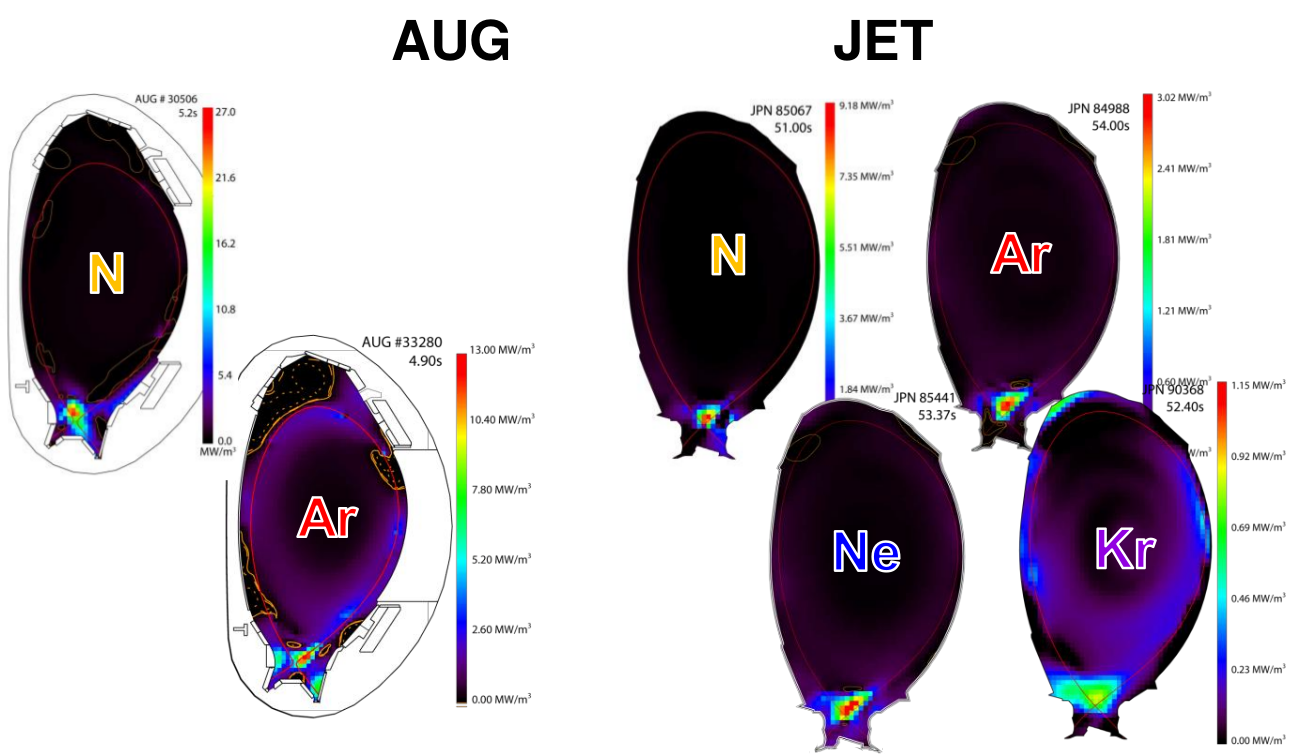
\includegraphics[width=\linewidth]{Chapters/chapter1/figs/xprs.png}
	\caption{Different radiation profiles with clear presence of X-point radiator for different impurities
	\cite{Wiesen2017}}
	\label{fig:xprs}
\end{figure}

The X-point radiator cannot be idealised as easily as the thermal front of detachment, because it is much more related to core and edge dynamics. Modeling its behaviour requires the use of codes that accounts for all atomic interactions, drifts, etc. like SOLPS-ITER, EDGE2D-EIRENE, SOLEDGE2D-EIRENE [\cite{Wiesen2017a} and references therein]. The presence of the radiator significantly affects temperature, pressure and density distribution, especially in the pedestal, therefore it is likely to have an effect on the current distribution and MHD activity.
In the last years a large effort has been put forward in the characterisation of the behaviour of the X-point radiator and its macroscopic effects on the core / edge. This has been done mostly in conventional geometry tokamaks, both with metal and carbon wall.


\section{ELMs and XPR}
Another important feature of the XPR is the reduction in amplitude of ELMs. This can be attributed to the fact that the energy associated with it first heats up the radiator and then moves toward the target. If the neutral density between X-point and target, and in the radiator itself, is high enough it could be possible to avoid ELMs to “burn through” the detachment front and to reach the target altogether. \cite{Krasheninnikov2016}



\section{Analytic models}\label{Analytic models}

In order to qualify and characterise the evolution of detachment it is useful to build approximate analytical models for the properties of interest, like particle and power fluxes, depending of the upstream plasma conditions. The most widely model is the two point model (2PM) and its variations.\cite{Stangeby2001} In it the complex 3D geometry of the SOL is translated to a simpler 1D system as shown in \autoref{fig:2PM}.

\begin{figure}
	\centering
	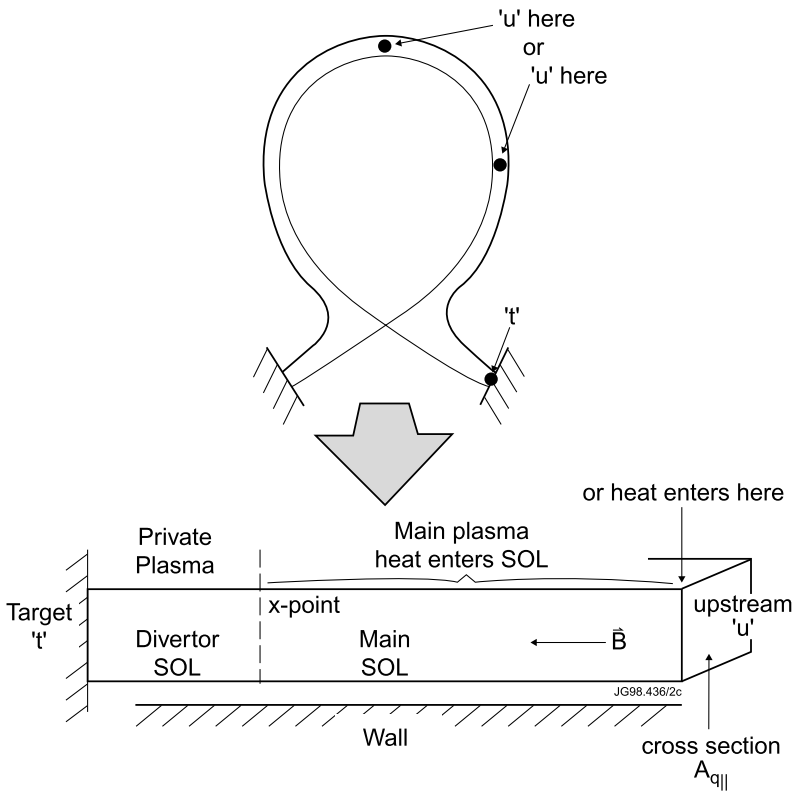
\includegraphics[trim={0 0 0 0},clip,width=0.65\linewidth]{Chapters/chapter1/figs/2PM.png}
	\caption{Schematic of how the poloidal SOL geometry can be straightened into a 1D one. The model is weakly sensitive to the location of the upstream location, assuming gradients are weak far from the divertor.\cite{Verhaegh2018} Adapted from \cite{Harrison2011} and the JET image database.}
	\label{fig:2PM}
\end{figure}

Then a series of assumptions are done:
\begin{itemize}
    \item There are no power losses along the SOL, excluding all radiated power losses.
    \item Ionisation does not affect the energy and flow profile.
    \item Heat is transported only via parallel heat conduction.
    \item Plasma pressure is considered constant in the entire SOL.
    \item Quasi neutrality and same temperature for electrons and ions ($n_e = n_i = n$, $T_e = T_i = T$).
    \item All the power to the SOL is transferred at the upstream location.
\end{itemize}

At the target surface the presence of the sheath accelerate the ions to the sound speed, so the local pressure given by the static and dynamic component $p_t$ is

\begin{equation}
p_{t} = p_{static} + p_{dynamic} = 2n_{t} k T_{t} + n_{t} m_i {{c_s}_t}^2
\label{eq:2pm1}
\end{equation}

Upstream the velocity component to the pressure is negligible so $p_u \approx 2 n_u k T_u$ so considering the pressure is uniform this returns the first equation of the 2PM

\begin{equation}
2 n_u k T_u = 2n_{t} k T_{t} + 2n_{t} k T_{t} \rightarrow n_u T_u = 2n_{t}T_{t}
\label{eq:2pm2}
\end{equation}

Since no volumetric power loss is considered the heat transferred to the SOL streams freely to the target, and it is determined by the sheath as

\begin{equation}
q_{\parallel} =  \gamma n_t k T_t {c_s}_t = \gamma n_t \sqrt{\frac{2(kT_t)^3}{m_i}}
\label{eq:2pm3}
\end{equation}
returning the second equation of the 2PM.

This heat is carried to the target via conduction. In order to calculate it, one should consider that the parallel heat conductivity for charged particles self-collisions can be written as ${v_{th}}_s mfp_s \approx {{v_{th}}_s}^2/{\nu_s}$ with ${v_{th}}_s$ the unidirectional thermal velocity of the species $s$, $mfp_s$ the self-collision mean free path and $\nu_s$ the self-collision frequency. ${v_{th}}_s$ is given by $\sqrt{8kT_s/{m_s}}$ while $\nu_s$ is proportional to $n_s/\sqrt{m_s T_s^3}$. The heat conductivity is then proportional to $ {T_s}^{5/2} / {m_s}^{1/2}$. This indicates that, given the mass difference, electrons dominate the conduction heat transfer, and that there is a strong dependency on the temperature. The heat flux can then finally be written as per \autoref{eq:2pm4a} where the electron parallel heat conductivity coefficient $\kappa$ is of the order of 2000.\cite{Stangeby2001}

\begin{equation}
q_{\parallel} = -\kappa T^{5/2} \frac{dT}{ds_{\parallel}}
\label{eq:2pm4a}
\end{equation}

This equation can be integrated from upstream to target (amounting to the connection length $L$), and considering that $q_{\parallel}$ is constant one can obtain the last equation of the 2PM model

\begin{equation}
{T_u}^{7/2} = {T_t}^{7/2} + \frac{7 q_{\parallel} L}{2 \kappa}
\label{eq:2pm4}
\end{equation}

Assuming fixed $q_{\parallel}, L, \gamma, m_i$ \autoref{eq:2pm2}, \ref{eq:2pm3} and \ref{eq:2pm4} contain 4 unknowns ($n_t, n_u, T_t, T_u$) and can be used to numerically solve for 3 when one is known or measured. If one assumes $T_u >> T_t$ as it is the case in the conduction limited regime, \autoref{eq:2pm4} can be further simplified neglecting $T_t$ and the 2PM reduces to

\begin{equation}
\begin{aligned}
T_t =& \frac{{q_{\parallel}}^2}{{n_u}^2 {T_u}^2} \; \frac{2m_i}{\gamma^2} \\
n_t =& \frac{{n_u}^3 {T_u}^3}{{q_{\parallel}}^2} \; \frac{\gamma^2}{4m_i} \\
T_u =& \left( \frac{7 q_{\parallel} L}{2 \kappa} \right)^{2/7}
\end{aligned}
\label{eq:2pm5}
\end{equation}

The target particle flux can finally be calculated as the heat flux over the energy released by each particle (neglecting the energy from surface recombination) from \autoref{eq:2pm3} as per \autoref{eq:2pm6} (the arrow refers to the further simplification as per \autoref{eq:2pm5}).

\begin{equation}
\Gamma_t = \frac{q_{\parallel}}{\gamma T_t} =  n_t \sqrt{\frac{2kT_t}{m_i}} \rightarrow \frac{{n_u}^2 {T_u}^2}{q_{\parallel}} \; \frac{\gamma^2}{2m_i}
\label{eq:2pm6}
\end{equation}
This correlation is the one that have been used in the literature to find detachment. The particle flux from Langmuir probes and the expectation from this scaling roughly match for an attached target. Increasing the upstream density further the particle flux plateaus then starts to decrease, deviating from the expected trend. This can be quantified in the Degree of Detachment (DoD) given by the ratio of the two quantities.\cite{Stangeby2001,Loarte1998}

This simple model can then be improved by including more of the true physics of the divertor and SOL like: volumetric power and momentum losses due to interactions with neutrals, volumetric radiated power losses, variation in $q_{\parallel}$ and pressure along field lines, sharp transition regions from x-point to target (e.g. ionisation / density / radiation front), magnetic configuration, etc.\cite{Stangeby2001,Cowley2022,Reinke2017,Lipschultz2016} This increase of sophistication allows, depending on the model, to also study the conditions along the leg, to investigate the relevance of different phenomena and the stability of the fronts movement. The fronts stability is particularly important because, as detached scenarios are more and more expected to provide the volumetric dissipation required for the target survival, it is paramount to be able to control their location. It has also been demonstrated that the threshold for rollover is proportional to a certain value of the ratio $ \frac {q_{rec}} {p_{up}}$ ($q_{rec}$ is the specific energy flux into the hydrogen recycling region). \cite{Krasheninnikov1999,Krasheninnikov2016,Stangeby2018}

Of relevance for the present work is that the depth of detachment increases with upstream density. This will be used to characterise density ramps in MAST-U during the first experimental campaign (MU01).







\section{Goals and objectives of the thesis}

\subsection{XPR/radiation front location and confinement (maybe the dataset is not there)}
find limit where confinement is not compromised, correlation between confinement and XPR/radiation location
\subsection{poloidal (toroidal?) divertor after XPR}
radiation spreading over all the separatrix, trasforming it into a limiter for the plasma.
\hl{I never observed this, is it worth mentioning?}
\subsection{XPR/detachment and power balance}
radiator location vs radiated power
\subsection{radiation front location and analytic models}
DOD vs radiator location, radiation front range/stability vs prediction
\subsection{detachment and configuration (CD/SXD)}
radiated power vs configuration (against predictions)
\subsection{radiation location and other metric of detachment}
radiator location vs MWI/LP compared to expectations, ionisation/MAR/recombination region (Kevin work)
\subsection{XPR and ELMs}
ELMs burn through/impact on LP and IR vs detachment/radiation front location
\subsection{Cyd Cowley paper}
hysteresis in inner leg detachment
\subsection{ELMs baffled in linear machine}
Magnum work, it is possible to prevent ELMs to reach the target with target pressure
\subsection{atomic vs molecular effects during ELMs burn through in deep detachment in linear machine}






